%%%%%%%%%%%%%%%%%%%%%%%%%%%%%%%%%%%%%%%%%
% a0poster Portrait Poster
% LaTeX Template
% Version 1.0 (22/06/13)
%
% The a0poster class was created by:
% Gerlinde Kettl and Matthias Weiser (tex@kettl.de)
% 
% This template has been downloaded from:
% http://www.LaTeXTemplates.com
%
% License:
% CC BY-NC-SA 3.0 (http://creativecommons.org/licenses/by-nc-sa/3.0/)
%
%%%%%%%%%%%%%%%%%%%%%%%%%%%%%%%%%%%%%%%%%

%-----------------------------------------------------------------------------
%	PACKAGES AND OTHER DOCUMENT CONFIGURATIONS
%-----------------------------------------------------------------------------
\pdfminorversion=4
\documentclass[a0,landscape]{a0poster}

%% % sans-serif config:


\usepackage[english]{babel}
\usepackage[utf8]{inputenc}
\usepackage[T1]{fontenc}
\renewcommand{\familydefault}{\sfdefault}

\usepackage{multicol} % This is so we can have multiple columns of
                      % text side-by-side
\columnsep=100pt % This is the amount of white space between the
                 % columns in the poster
\columnseprule=3pt % This is the thickness of the black line between
                   % the columns in the poster

\usepackage[svgnames]{xcolor} % Specify colors by their 'svgnames',
                              % for a full list of all colors
                              % available see here:
                              % http://www.latextemplates.com/svgnames-colors

\usepackage{tgheros}


%% \usepackage{times} % Use the times font
%% \usepackage{palatino} % Uncomment to use the Palatino fon

\usepackage{graphicx} % Required for including images
\usepackage{overpic}
\graphicspath{{figures/}} % Location of the graphics files
\usepackage{booktabs} % Top and bottom rules for table
\usepackage[font=small,labelfont=bf, format=hang]{caption} % Required for
                                              % specifying captions to
                                              % tables and figures
\usepackage{amsfonts, amsmath, amsthm, amssymb} % For math fonts,
                                                % symbols and
                                                % environments
\usepackage{wrapfig} % Allows wrapping text around tables and figures

%\usepackage{sfmath}
\usepackage[eulergreek]{sansmath} %additional math
\sansmath

\usepackage{mathsetup}

\usepackage{bibconfig}

\usepackage{titlesec}

\usepackage{siunitx}
\sisetup{detect-all}

\titlespacing*{\section}
{0pt}{2.5ex plus 1ex minus .2ex}{1.5ex plus .2ex}


\makeatletter
\g@addto@macro\normalsize{%
  \setlength\abovedisplayskip{18pt}
  \setlength\belowdisplayskip{18pt}
  \setlength\abovedisplayshortskip{16pt}
  \setlength\belowdisplayshortskip{16pt}
}
\makeatother


\addtolength{\parskip}{0.5\baselineskip}
\parindent 0pt

\definecolor{gblue}{RGB}{27,98,183}

\begin{document}

%-----------------------------------------------------------------------------
%	POSTER HEADER 
%-----------------------------------------------------------------------------

% The header is divided into two boxes:
% The first is 75% wide and houses the title, subtitle, names, university/organization and contact information
% The second is 25% wide and houses a logo for your university/organization or a photo of you
% The widths of these boxes can be easily edited to accommodate your content as you see fit
%\vspace{-6cm}

%\fbox{
\begin{minipage}[b]{0.75\linewidth}
\vspace{-0.5cm}   
  \veryHuge \textbf{Modelling synaptic lifetime distributions with Kesten processes} \color{Black}\\[1.5cm] 
%\Huge\textit{}\\[2cm] % Subtitle
  \huge \textbf{Felix Z.~Hoffmann$^{1,2}$, Daniel Miner$^{1,3}$, Jochen Triesch$^1$}\\[0.5cm] % Author(s)
\large $\quad ^1$ Frankfurt Institute for Advanced Studies (FIAS), Johann Wolfgang Goethe University, Frankfurt am Main, Germany\\[0.2cm] % University/organization
$\quad ^2$ International Max Planck Research School for Neural Circuits, Max Planck Institute for Brain Research, Frankfurt am Main, Germany\\[0.2cm]
$\quad ^3$ Third Institute of Physics, Universität Göttingen, Göttingen, Germany
\\[0.4cm]
\end{minipage}
%}
%
%\fbox{
\begin{minipage}[b]{0.25\linewidth}
  \centering
  
  %% 
\includegraphics[width=10cm]{goethe-logo.pdf}\\
  %% \vspace{2.8cm}
  \vspace{-9cm}
  
  
\includegraphics[width=11cm]{spp2041_logo.pdf}
  \hspace{2.2cm}
  
\includegraphics[width=12.5cm]{FIAS-logo.pdf}\\

  \vspace{2cm}
  \Large \texttt{hoffmann@fias.uni-frankfurt.de}\\
  \vspace{3cm}
\end{minipage}
%}
\vspace{-1.5cm} % A bit of extra whitespace between the header and poster content

%-----------------------------------------------------------------------------

\begin{multicols}{3} % This is how many columns your poster will be
                     % broken into, a portrait poster is generally
  % split into 2 columns
  \section{Introduction}
\vspace{-0.2cm}

The wiring of cortical circuits is highly dynamic. Spine sizes fluctuate even in the absence of neural activity and there is constant synaptic turnover \cite{Loewenstein2015}. In models of cortical circuits, two major mechanisms are typically considered to drive the efficacies of synaptic connections: Spike-timing dependent plasticity (STDP) is often assumed to strengthen or weaken synaptic connections in an additive manner, independent of the current weight. Synaptic normalization, on the other hand, acts multiplicatively on synapses by scaling their efficacies by a varying factor that depends on the availability of synaptic resources \cite{Triesch2017} (see Fig.~\ref{fig:spines}).



\begin{center}\vspace{0.01cm}
  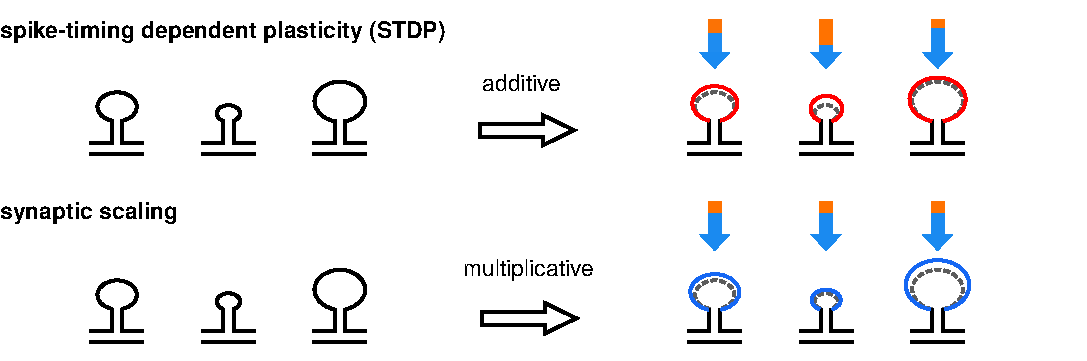
\includegraphics[width=\columnwidth]{%
    /home/fh/pub/graphics/synapse_size_dynamics/synapse_size_dynamics.png} %
  \captionof{figure}{Spike-timing dependent plasticity changes synaptic efficacies additively, while synaptic normalization acts multiplicatively on the synaptic weights.}
  \label{fig:spines}
\end{center}\vspace{2cm}


To model the fluctuations of synaptic spine sizes over time, a stochastic process called Kesten process has been suggested \cite{Kesten1973, Statman2014}. In this process, a random variable $X_n$ at time step $n$ is updated by scaling it with a random multiplicative factor $a_n$ and then adding a random increment $b_n$ according to
%
\begin{align}
  X_{n+1} = a_n X_n + b_n. \label{eq:kesten}
\end{align}
%
This stochastic model has been successfully used to describe the distribution of synaptic spine sizes measured in experiments. Here we extend the Kesten process by including the explicit creation and elimination of spines. Simulation and analysis of the model reveals that the distribution of lifetimes approximately follow a power law, as has been recently identified in experiments in the rat neocortex \cite{Loewenstein2015}.


%% In an experimental study by \textcite{Loewenstein2015} chronic in-vivo two-photon imaging suggested that the lifetime dynamics of spines in the neocortex follow a power law. Motivated by results from detailed network simulations, we here consider a simple stochastic model based on the Kesten process in order to analyze how different properties of a cortical network might affect the lifetime distributions of synaptic spines.

  
%\vspace{-0.4cm}
\section*{Model}
\vspace{-0.2cm}

We consider a Kesten process $X_n$ that models spine size dynamics. A given spine size $X_n$ at time step $n$ is updated as $X_{n+1} = a_n X_n + b_n$ as in \eqref{eq:kesten}. Here, both $a_n$ and $b_n$ are drawn randomly at each time step from a normal distribution, $a_n \sim \mathcal{N}(\mu_a, \sigma_a^2)$ and $b_n \sim \mathcal{N}(\mu_b, \sigma_b^2)$. To model synapse growth and pruning processes, we consider a population of $N$ synapses. Each synapse has a random time $T_{\mathrm{init}}$, uniformly distributed in $[0,T_{\text{max}}]$, at which it is initialized with size $X_0$. The synaptic spine size $X_t$ then evolves according to \eqref{eq:kesten}.

\begin{minipage}{\columnwidth}
  \begin{center}
    \vspace{0.75cm}
  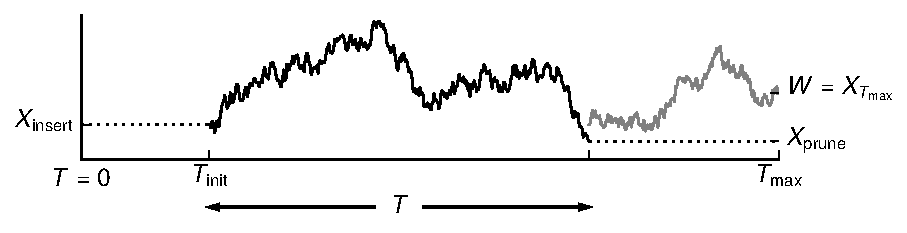
\includegraphics[width=0.95\columnwidth]{%
    figures/abstract_fig.pdf}
  %% /home/fh/sci/lab/syn_lt/kesten_model/note_x/km_ca_rts_dd/img/abstract_fig.png}
  \captionof{figure}{Adapted Kesten simulation model allows the tracking of lifetimes and size distributions}
  \label{fig:km}
\end{center}
\end{minipage}

\columnbreak
The lifetime of a synapse is the number of time steps from $T_{\text{init}}$ until for the first time $X_t < X_{\mathrm{prune}}$, where $X_{\mathrm{prune}}$ is a fixed parameter smaller than $X_0$ for the population. In this event the synapse gets pruned and a new synapse with size $X_0$ is inserted in the network (Fig.~\ref{fig:km}). In the case that $X_t$ doesn't fall below $X_{\mathrm{prune}}$ until $T_{\text{max}}$, the lifetime is recorded as $T=T_{\text{max}}-T_{\text{init}}$. At the end of the simulation the sizes $X_{T_{\text{max}}}$ are recorded for all $N$ synapses.


  \section*{Results}

We simulated $N= \,\,$\SI{5e5} synapses evolving as Kesten processes and recorded lifetime and weight distributions. First, we systemically tested the effect of the distribution parameters on lifetime and weight distributions. We found that within parameter ranges as for example used in the Kesten model of \textcite{Statman2014}, the variance of the multiplicative component $\sigma_a^2$ has negligible effect on lifetime and weight distributions.

This allowed us to further reduce the Kesten model in complexity and allowed us consider to an autoregressive AR(1) process of the form
%
\begin{align}
  X_{n+1} = a\, X_n + b_n,
\end{align}
%
where $a \in (0,1)$ and $b_n \sim \mathcal{N}(\mu_b, \sigma_b^2)$ instead.
For unbiased additive change ($\mu_b =0$), a power law like distribution of synaptic lifetimes emerges (Fig.~\ref{fig:lifetimes}A). The distribution of spine sizes $X_{T_{\text{max}}}$ resembles a log-normal distribution, as one might expect from findings on the synaptic weight distributions in cortical circuits \cite{Song2005}.

\vspace{1.2cm}
\begin{overpic}[width=\columnwidth]%
  % 110, 133
  {figures/lifetimes_weights.pdf}
  %\put(32,\ylin){anisotropic}
  \put(1,28){\normalfont \textbf{A}}
  \put(52,28){\normalfont \textbf{B}}
\end{overpic}
\captionof{figure}[format=hang,indention=1cm]{Dynamical properties of network connectivity modelled by Kesten processes. \textbf{A} Lifetime distribution of synapses created at time step $T_{\text{init}}$ uniformly distributed in $[0, T_{\text{max}}]$. \textbf{B} Distribution of spine sizes $X_{T_{\text{max}}}$ at time step $X_{T_{\text{max}}}$ (grey) and log-normal fit (red). Parameters for both: $a=0.9987$, $\mu_b=0$, $\sigma_b^2=0.22$, $X_{\text{insert}}=0.1$, $X_{\text{prune}}=0.01$. \label{fig:lifetimes}}

\vspace{3cm}

%% \begin{center}\vspace{1cm}
%%   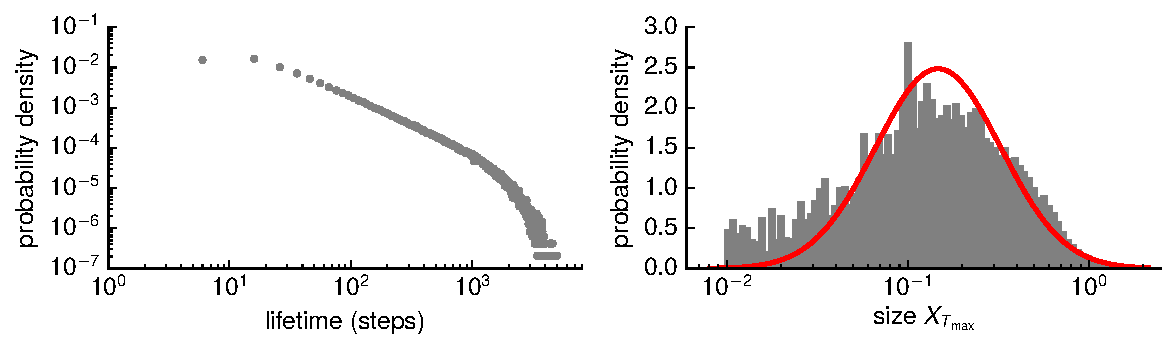
\includegraphics[width=\columnwidth]{%
%%     %% /home/fh/sci/lab/syn_lt/kesten_model/note_x/km_ca_rts_dd/img/lifetimes_weights.png}
%%     figures/lifetimes_weights.png}

%%   \captionof{figure}{}
%%   \label{fig:lifetimes}
%% \end{center}\vspace{1cm}

Next, we explored how different parameters in the model affect the lifetime and spine size distributions. We found that varying $\sigma_b^2$ has little effect on the distributions. Interestingly however, the bias in the additive change affects both distributions significantly. As one might expect, a bias towards increases in size moves the tail of the lifetime distribution towards higher lifetimes (Fig.~\ref{fig:lifemub}A) while shifting the mean of the spine size towards higher values (Fig.~\ref{fig:lifemub}B). This observation matches qualitatively with preliminary results from detailed network simulations in which a higher bias towards LTP resulted in similarly extended lifetimes.

  \vspace{1.4cm}
\begin{overpic}[width=\columnwidth]%
  % 110, 133
  {figures/lifetimes_weights_mub_compare_logweight.pdf}
  %\put(32,\ylin){anisotropic}
  \put(1,28){\normalfont \textbf{A}}
  \put(52,28){\normalfont \textbf{B}}
\end{overpic}
  \captionof{figure}{The bias of additive change in size strongly affects both lifetime and weight distributions. \label{fig:lifemub}}

  \vspace{1.8cm}

    
\section{Network simulations}

\vspace{1.4cm}
\begin{overpic}[width=\columnwidth]%
  % 110, 133
  {figures/lifetimes_single.pdf}
  %\put(32,\ylin){anisotropic}
  \put(1,28){\normalfont \textbf{A}}
  \put(52,28){\normalfont \textbf{B}}
\end{overpic}
  \captionof{figure}{The bias of additive change in size strongly affects both lifetime and weight distributions. \label{fig:netwsim}}


\vfill

  \section{Key points}

\begin{itemize}
\item[-] For lifetime and size distributions, Kesten process can be reduced to simpler autoregressive AR(1) process
\item[-] Lifetime distributions in the model approximately follow a power law as observed experimentally
\item[-] In both the stochastic model and detailed network simulations the bias in the additive changes in synaptic weight systematically shapes the lifetime distributions
\item[-] Increased noise results in both model and network simulation 
\end{itemize}
                        

  
  \printbibliography  

\end{multicols}

%% \begin{columns}
%%   %
%%   \begin{column}{.5\textwidth}
%%     \input{sections/abstract}  
%% \section{Introduction}
\vspace{-0.2cm}

The wiring of cortical circuits is highly dynamic. Spine sizes fluctuate even in the absence of neural activity and there is constant synaptic turnover \cite{Loewenstein2015}. In models of cortical circuits, two major mechanisms are typically considered to drive the efficacies of synaptic connections: Spike-timing dependent plasticity (STDP) is often assumed to strengthen or weaken synaptic connections in an additive manner, independent of the current weight. Synaptic normalization, on the other hand, acts multiplicatively on synapses by scaling their efficacies by a varying factor that depends on the availability of synaptic resources \cite{Triesch2017} (see Fig.~\ref{fig:spines}).



\begin{center}\vspace{0.01cm}
  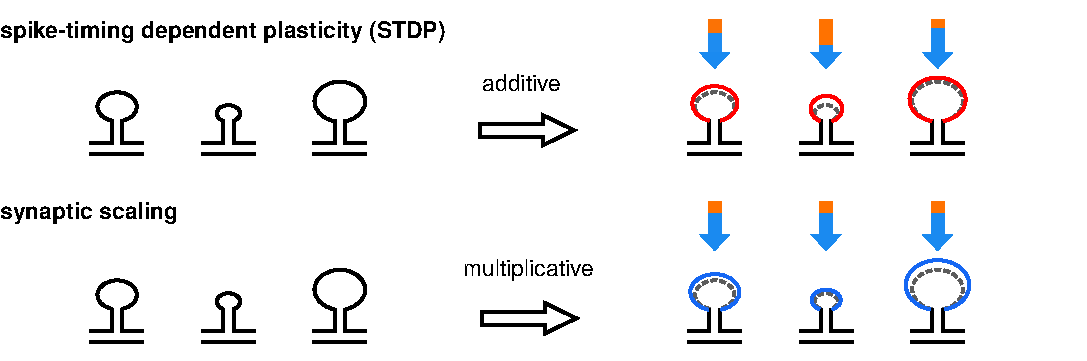
\includegraphics[width=\columnwidth]{%
    /home/fh/pub/graphics/synapse_size_dynamics/synapse_size_dynamics.png} %
  \captionof{figure}{Spike-timing dependent plasticity changes synaptic efficacies additively, while synaptic normalization acts multiplicatively on the synaptic weights.}
  \label{fig:spines}
\end{center}\vspace{2cm}


To model the fluctuations of synaptic spine sizes over time, a stochastic process called Kesten process has been suggested \cite{Kesten1973, Statman2014}. In this process, a random variable $X_n$ at time step $n$ is updated by scaling it with a random multiplicative factor $a_n$ and then adding a random increment $b_n$ according to
%
\begin{align}
  X_{n+1} = a_n X_n + b_n. \label{eq:kesten}
\end{align}
%
This stochastic model has been successfully used to describe the distribution of synaptic spine sizes measured in experiments. Here we extend the Kesten process by including the explicit creation and elimination of spines. Simulation and analysis of the model reveals that the distribution of lifetimes approximately follow a power law, as has been recently identified in experiments in the rat neocortex \cite{Loewenstein2015}.


%% In an experimental study by \textcite{Loewenstein2015} chronic in-vivo two-photon imaging suggested that the lifetime dynamics of spines in the neocortex follow a power law. Motivated by results from detailed network simulations, we here consider a simple stochastic model based on the Kesten process in order to analyze how different properties of a cortical network might affect the lifetime distributions of synaptic spines.


%%   \end{column}
%%   %
%%   \begin{column}{.5\textwidth}

%%       \section*{Results}

We simulated $N= \,\,$\SI{5e5} synapses evolving as Kesten processes and recorded lifetime and weight distributions. First, we systemically tested the effect of the distribution parameters on lifetime and weight distributions. We found that within parameter ranges as for example used in the Kesten model of \textcite{Statman2014}, the variance of the multiplicative component $\sigma_a^2$ has negligible effect on lifetime and weight distributions.

This allowed us to further reduce the Kesten model in complexity and allowed us consider to an autoregressive AR(1) process of the form
%
\begin{align}
  X_{n+1} = a\, X_n + b_n,
\end{align}
%
where $a \in (0,1)$ and $b_n \sim \mathcal{N}(\mu_b, \sigma_b^2)$ instead.
For unbiased additive change ($\mu_b =0$), a power law like distribution of synaptic lifetimes emerges (Fig.~\ref{fig:lifetimes}A). The distribution of spine sizes $X_{T_{\text{max}}}$ resembles a log-normal distribution, as one might expect from findings on the synaptic weight distributions in cortical circuits \cite{Song2005}.

\vspace{1.2cm}
\begin{overpic}[width=\columnwidth]%
  % 110, 133
  {figures/lifetimes_weights.pdf}
  %\put(32,\ylin){anisotropic}
  \put(1,28){\normalfont \textbf{A}}
  \put(52,28){\normalfont \textbf{B}}
\end{overpic}
\captionof{figure}[format=hang,indention=1cm]{Dynamical properties of network connectivity modelled by Kesten processes. \textbf{A} Lifetime distribution of synapses created at time step $T_{\text{init}}$ uniformly distributed in $[0, T_{\text{max}}]$. \textbf{B} Distribution of spine sizes $X_{T_{\text{max}}}$ at time step $X_{T_{\text{max}}}$ (grey) and log-normal fit (red). Parameters for both: $a=0.9987$, $\mu_b=0$, $\sigma_b^2=0.22$, $X_{\text{insert}}=0.1$, $X_{\text{prune}}=0.01$. \label{fig:lifetimes}}

\vspace{3cm}

%% \begin{center}\vspace{1cm}
%%   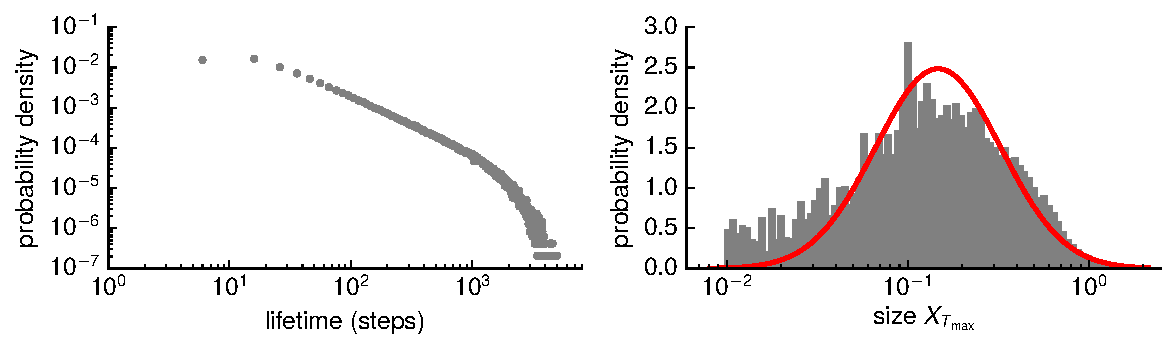
\includegraphics[width=\columnwidth]{%
%%     %% /home/fh/sci/lab/syn_lt/kesten_model/note_x/km_ca_rts_dd/img/lifetimes_weights.png}
%%     figures/lifetimes_weights.png}

%%   \captionof{figure}{}
%%   \label{fig:lifetimes}
%% \end{center}\vspace{1cm}

Next, we explored how different parameters in the model affect the lifetime and spine size distributions. We found that varying $\sigma_b^2$ has little effect on the distributions. Interestingly however, the bias in the additive change affects both distributions significantly. As one might expect, a bias towards increases in size moves the tail of the lifetime distribution towards higher lifetimes (Fig.~\ref{fig:lifemub}A) while shifting the mean of the spine size towards higher values (Fig.~\ref{fig:lifemub}B). This observation matches qualitatively with preliminary results from detailed network simulations in which a higher bias towards LTP resulted in similarly extended lifetimes.

  \vspace{1.4cm}
\begin{overpic}[width=\columnwidth]%
  % 110, 133
  {figures/lifetimes_weights_mub_compare_logweight.pdf}
  %\put(32,\ylin){anisotropic}
  \put(1,28){\normalfont \textbf{A}}
  \put(52,28){\normalfont \textbf{B}}
\end{overpic}
  \captionof{figure}{The bias of additive change in size strongly affects both lifetime and weight distributions. \label{fig:lifemub}}

  \vspace{1.8cm}

%%   \end{column}
%% \end{columns}


\end{document}
